\chapter{Model}\label{sec:model}
\section{ResNet18 architecture trained with MixUp}
On the Kaggle classification competetion related to the HAM10000 dataset\cite{HAM10000-kaggle-competetion},
another user claimed to get a $97.7\%$ Multi-class accuracy using a ResNet18 model trained with MixUp 
(explained in Section \ref{sec:mixup})\cite{kaggle-97-model}.
When the provided model was retrained,
the results were not as good as claimed.
The actual accuracy was in the range of $90\%$ to $92\%$,
depending on the data split.
That is however still close to the best performing model published (see \ref{sec:state-of-the-art}).

The actual implementation of the model can be seen in Appendix \ref{appendix:resnet-18-mixup}.
Using the slight modifications to the original mode, the model reached an accuracy of roughly $91.5\%$.

\subsection{Data augmentation}
To compensate for the fairly small size of the dataset,
multiple different kinds of data augmentation was used.
These are explained in the following sections.
\subsubsection{Resize}
To standardize all the images, the images were resized to $450\times450$ pixels.

\subsubsection{MixUp} \label{sec:mixup}
MixUp is a technique to among other nice side effects minimize overfitting when training 
an image classification model.
The idea is to do weighted averaring of both the images and their labels.
In this case, we simply combine pairs of images and take their average.
The same goes for their labels, that are expected to be one-hot encoded.
For instance if two images from a $3$-class classification problem had labels $[0,0,1]$ and $[1,0,0]$,
the resulting label would be $[0.5,0.5,0]$.
On Figure 
\begin{figure}
    % Make three subfigures
    %\includegraphics[width=0.3\textwidth]{build/data_aug_examples/image_A.jpg}
    \begin{subfigure}{0.3\textwidth}
        \includegraphics[width=\textwidth]{build/data_aug_examples/image_A.jpg}
        \caption{Image A}
        \label{fig:image-A}
    \end{subfigure}
    \begin{subfigure}{0.3\textwidth}
        \includegraphics[width=\textwidth]{build/data_aug_examples/image_B.jpg}
        \caption{Image B}
    \end{subfigure}
    \begin{subfigure}{0.3\textwidth}
        \includegraphics[width=\textwidth]{build/data_aug_examples/image_A_mixup.jpg}
        \caption{Image A mixed with Image B}
    \end{subfigure}
    \captionof{figure}{Example two images of skin lesions mixed using MixUp}
    \label{fig:mixup-example}
\end{figure}

MixUp as a data augmentation technique has been shown to increase the accuracy of models \cite{mixup-paper}.
It does however come with the downside, that it is computationally expensive,
since a lot of epocs are needed for it to work effectively.

\subsubsection{Rotation and Flip}
The images were rotated and flipped to increase the dataset size.
Since it should matter which side an image is captured from, 
the rotation shouldn't matter to a perfect model.
For the same reason, neither should a mirrored image.
Examples of how this works can be seen in Figure \ref{fig:dihedral-flip-examples}.
\begin{center}
    \includegraphics[width=0.8\textwidth]{./build/data_aug_examples/dihedral_flip_examples.png}
    \captionof{figure}{Example of an image of a lesion flipped and rotated in all possible combinations.}
    \label{fig:dihedral-flip-examples}
\end{center}

\subsubsection{Cropping}
Since fills out most of the image,
it shouldn't matter a lot if the image is cropped.
The images are cropped such that between $75\%$ and $100\%$ of the image is visible.
The crop is then made on a random location of the image.
An example of this can be seen in Figure \ref{fig:cropping-example}

\begin{center}
    \includegraphics[width=0.3\textwidth]{./build/data_aug_examples/image_A_crop.jpg}
    \captionof{figure}{Image of the lesion in Figure \ref{fig:image-A} cropped.}
    \label{fig:cropping-example}
\end{center}



\section{The HAM10000 dataset}
The HAM10000 dataset contains 10015 images of skin lesions.
These images are a subset of the images from the ISIC dataset\cite{ISIC_Dataset_2018},
which collects images of skin lesions and hosts annual competitions for skin lesion diagnosis.
They are divided into seven classes as seen in the Table \ref{table:ham10000}.
A \textit{severity} has also been assigned each class.
These indicate if the lesion class benign, malignant or pre-malignant.
Malignant tumors are those where the cells are replicationg uncontrollably,
and there is a risk of these cells spreading to the rest of the body.
Beningn tumors can still hurt the patient, but are much less of a worry,
as they are not replicationg uncontrollably and hence do not lead to cancer.

\begin{table}[ht]
\begin{center}
\begin{tabular}{|c|c|c|c|c|c|c|}
\hline
Label    & Name                          & Severity      & Dataset prevalence \\ \hline
akiec    & Bowens disease                & pre-malignant & $3.27\%$           \\ \hline
nv       & Melanocytic nevi              & benign        & $66.94\%$          \\ \hline
mel      & Melanoma                      & malignant     & $11.11\%$          \\ \hline
bkl      & Benign keratosis-like lesions & benign        & $10.97\%$          \\ \hline
bcc      & Basal cell carcinoma          & malignant     & $5.13\%$           \\ \hline
vasc     & Vascular lesions              & benign        & $1.41\%$           \\ \hline
df       & Dermatofibroma                & benign        & $1.14\%$           \\ \hline
\end{tabular}
\end{center}

\caption{Overview of the HAM10000 dataset. The severity of lesions are taken from \cite{dermatologi-laerebogen}.}
\label{table:ham10000}
\end{table}

\subsection{State of the art models}\label{sec:state-of-the-art}
Due to the public nature of the dataset, many different models have been trained on it.
As of the time of writing, the best performing model published in a scientific paper,
reaches an accuracy of $93.4\%$\cite{datta2021soft}.

\subsection{Confounding elements in the data} \label{sec:confounding}
The dataset contains images of skin lesions, which are taken in a real world medical context.
In this context doctors might introduce foreign objects into the images,
to help in the treatment of the patient.
Examples of these can be seen on Figure \ref{fig:confounding_objects}.

\begin{figure}[ht]
    \begin{center}
        \begin{subfigure}[b]{0.3\textwidth}
            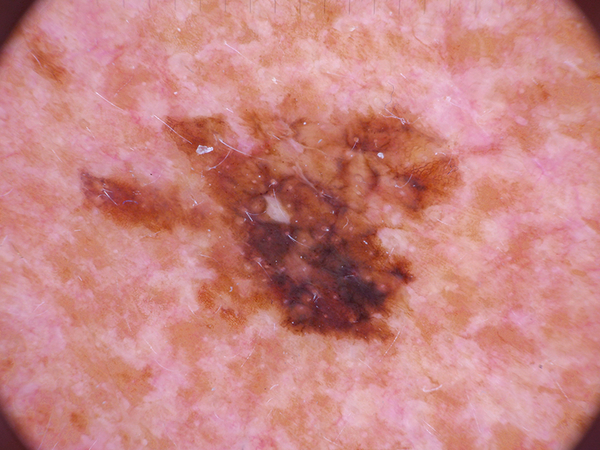
\includegraphics[width=\textwidth]{./images/ISIC_0024310.jpg}
            \caption{Image of skin lesion with black frame}
        \end{subfigure}
        \begin{subfigure}[b]{0.3\textwidth}
            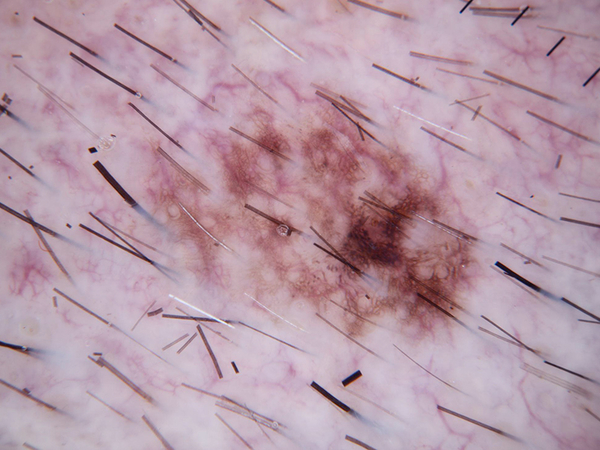
\includegraphics[width=\textwidth]{./images/ISIC_0024420.jpg}
            \caption{Image of skin lesion with ruler (upper right corner)}
        \end{subfigure}
        \begin{subfigure}[b]{0.3\textwidth}
            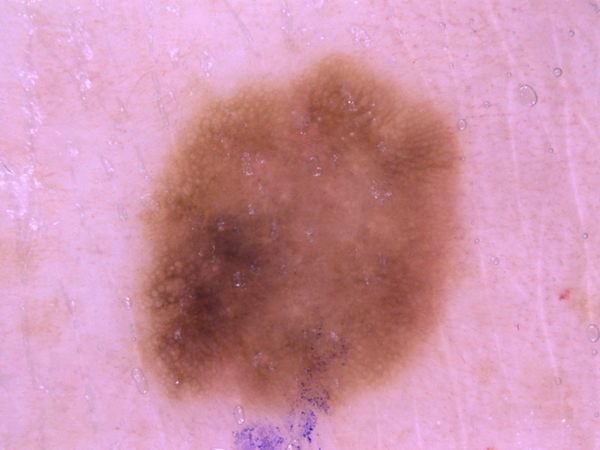
\includegraphics[width=\textwidth]{./images/ISIC_0027514.jpg}
            \caption{Image skin lesion with blue ink}
        \end{subfigure}
    \end{center}
    \caption{Images with different confounding objects}
    \label{fig:confounding_objects}
\end{figure}

Labeling some of these confounding objects, we see that the rulers occur way more often than the others with a prevalence of roughly $17\%$ (See Table \ref{table:confounding_objects}).
Due to this higher prevalence, the study done in this project will focus on the ruler markings over the other confounding objects.

\begin{table}
    \centering
    \begin{tabular}{|l|r|}
        % confounding_objects.ipynb
        \hline 
        Confounder &  Prevalence \\ \hline
        ruler   &  0.171842 \\ \hline
        sticker &  0.000100 \\ \hline
        ink     &  0.003495 \\ \hline
    \end{tabular}
    \caption{Dataset prevalence of confounding objects}
    \label{table:confounding_objects}
\end{table}

\subsection{Correlation between confounding elements and HAM10000 labels}
On Figure \ref{fig:ruler_vs_dx} indications of correlations between the ruler markings and the HAM10000 labels can be seen.

\begin{figure}[ht]

\centering
\includegraphics[width=0.8\textwidth]{./build/confounder_label_correlation/confusion_matrix_seaborn.png}
\caption{Pivot table of rulers vs. class in the HAM10000 dataset - normalized over the x-axis.}
\label{fig:ruler_vs_dx}
\end{figure}

The two benign classes \textit{mel} and \textit{bkl} are both over represented on pictures with ruler markings copared to those without.
In general almost every class except the biggest \textit{nv} class is over represented.
The hypothesis that the presence of rulers in the images is correlated with the HAM10000, can be confirmed by a $\chi^2$-contingency test.
The null hypothesis of this test is that the presence of rulers in the images is not correlated with the HAM10000 labels.
The test value is 
    $\input{build/confounder_label_correlation/chi2.txt}$
on a test with
    $\input{build/confounder_label_correlation/dof.txt}$
degrees of freedom, resulting in a $p$-value of 
    $\input{build/confounder_label_correlation/p.txt}$
which is obviously significant.

\begin{center}
    \includegraphics[
        width=0.7\textwidth,
    ]{build/prediction_strength/confusion_matrix_seaborn.png}
    \captionof{figure}{Confusion matrix of the model prediction on the dataset. 
        Normalization has been done over the truth.
    }
    \label{fig:prediction_strength}
\end{figure}

\section{Prediction precision on different classes}
The model is trained on $80\%$ of the data, and is tested on the remaining $20\%$.

In Figure \ref{fig:prediction_strength} a confusion matrix for the trained model tested on the test set is shown.
The metrics described in Section \ref{sec:model_metrics} calculated for the model can be seen in Table \ref{tab:resnet-model-metrics}.
\begin{table}
    \centering
    \input{build/segmented_prediction_strength/metrics_table.tex}
    \caption{Metrics for the model as evaluated on the $20\%$ test set.}
    \label{tab:resnet-model-metrics}
\end{table}